\section{Forschungsmethoden}
\label{cha:method}
In Abbildung~\ref{fig:einfluss_forschungsmethoden} ist dargestellt, wie die für diese Arbeit gewonnen Informationen in das Ergebnis eingeflossen sind. Auf Basis der 
Ergebnisse der systematischen Literaturübersicht wurde das Vorgehensmodell 
entwickelt. Anschließend wurde dieses theoretische Modell auf ein Projekt aus 
der Praxis angewandt, um ein modell-ideales Vorgehen aufzuzeigen. Zum Schluss 
wurde dieses ideale Vorgehen mit Erfahrungen aus der Praxis konfrontiert und 
erweitert.

\usetikzlibrary{decorations.text}
\usetikzlibrary{calc}
\usetikzlibrary{fit}
\usetikzlibrary{shapes}
\usetikzlibrary{arrows,positioning} 

%\begin{document}
\begin{figure}[h]
\begin{center}
\scalebox{1}{
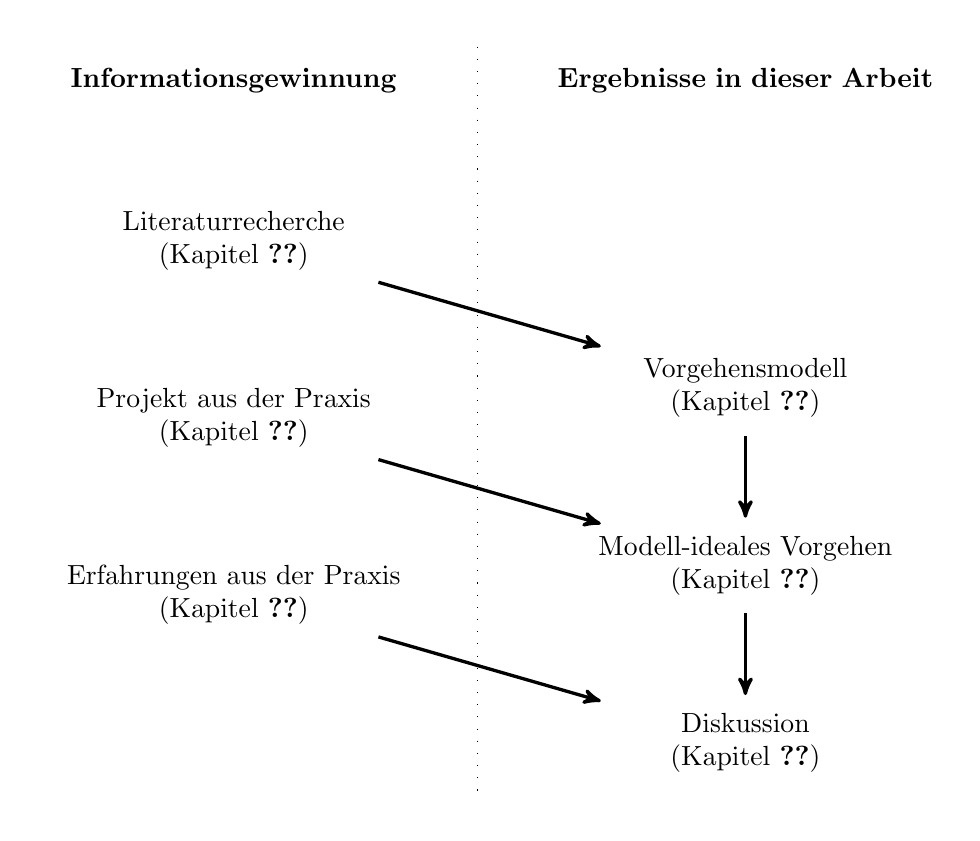
\begin{tikzpicture}[
	node distance=1.25cm,
	auto,
	pile/.style={
		very thick,
		->,
		>=stealth',
		shorten <=3pt,
		shorten >=3pt
	},
	knoten/.style={
		text width=5cm,
		text centered
	}
]
\node[knoten] (INFOS)  {\textbf{Informationsgewinnung}};
\node[knoten] (ERG) [right=of INFOS] {\textbf{Ergebnisse in dieser Arbeit}};

\node[knoten] (LIT) [below=of INFOS]
{Literaturrecherche\\(Kapitel~\ref{cha:literaturuebersicht})};

\node[knoten] (INV) [below=of ERG, right=of LIT] {};


\node[knoten] (PROJ) [below=of LIT] {Projekt aus 
der Praxis\\(Kapitel~\ref{cha:replyundifms})};

\node[knoten] (VOR) [right=of PROJ, below=of INV] 
{Vorgehensmodell\\(Kapitel~\ref{cha:entwicklung_vorgehensmodell})};


\node[knoten] (IDEAL) [below=of VOR] 
{Modell-ideales Vorgehen\\(Kapitel~\ref{cha:result})};

\node[knoten] (ERF) [below=of PROJ] {Erfahrungen aus 
der Praxis\\(Kapitel~\ref{cha:praxis})};

\node[knoten] (DISK) [below=of IDEAL] 
{Diskussion\\(Kapitel~\ref{cha:diskussion})};

\node[above left = 0.15cm and 0.65cm of ERG] (o) {};
\node[below left = 0.15cm and 0.65cm of DISK] (u) {};

\draw[loosely dotted] (o) -- (u);

\draw[pile] (LIT) -> (VOR);
\draw[pile] (VOR) -> (IDEAL);
\draw[pile] (PROJ) -> (IDEAL);
\draw[pile] (IDEAL) -> (DISK);
\draw[pile] (ERF) -> (DISK);

\end{tikzpicture}
}
\caption{Einfluss der Forschungsmethoden in die Arbeit}
\label{fig:einfluss_forschungsmethoden}
\end{center}
\end{figure}

Die Abläufe der systematischen Literaturrecherche und der Gespräche und 
Workshops werden in den 
Kapiteln~\ref{cha:literaturuebersicht}~beziehungsweise~\ref{cha:praxis} 
dargestellt. Das Praxisprojekt wurde bereits in Kapitel~\ref{cha:replyundifms} 
vorgestellt, weshalb auf eine erneute Vorstellung an dieser Stelle verzichtet 
wird.
\subsection{Theorie: Systematische Literaturübersicht}
\label{cha:literaturuebersicht}
Die systematische Literaturübersicht wurde wie von \citeflow{kitchenham2004} 
vorgeschlagen durchgeführt: Zunächst wurden für jede Forschungsfrage 
Schlüsselwörter und ihre Synonyme identifiziert und anschließend mit booleschen 
Operatoren verknüpft. Die entstandenen Ausdrücke sind in 
Tabelle~\ref{tab:searchstrings} zu finden und dienten anschließend der 
Recherche in den Literaturdatenbanken aus Tabelle~\ref{tab:literaturdatenbanken}.
%
% WICHTIG
% Wenn hier eine Frage angepasst wird, muss sie auch in der Datei 
% forschungsfragen.tex angepasst werden
%
\begin{table}[h]
\centering
\begin{tabular}{|l|p{0.35\textwidth}|p{0.55\textwidth}|}
	\hline
	\textbf{\#} & \textbf{Frage} & \textbf{Rechercheausdruck} \\
	\hline
	1 & In welche Aufgaben lässt sich die Migration 
einer On-Premise-Software zu Salesforce unterteilen? & (tasks OR 
needs OR requirements)\newline AND\newline (migration OR adoption)\newline 
AND\newline salesforce
\\
	\hline
	2 & Welche Methoden unterstützen diesen Migrationsprozess? & (methods OR 
standards OR framework) \newline AND\newline 
('cloud migration' OR 'cloud adaption' OR 'salesforce') \\
	\hline
	3 & Wie unterstützt Salesforce die Migration technisch? & (tools OR 
interfaces OR api)\newline AND\newline (migration OR 
adoption)\newline 
AND\newline salesforce\\
	\hline
	4 & Wie wirkt sich die Migration auf die strategische Marktposition aus? 
& (strategy OR market) \newline 
AND\newline 
('cloud migration' OR 'cloud adaption') \\
	\hline
\end{tabular}
\caption{Forschungsfragen und zugehörige Rechercheausdrücke. Angelehnt 
an \cite{exploring_the_factors}
}
\label{tab:searchstrings}
\end{table}



Ausgeschlossen und in der Tabelle vermerkt wurden Literaturdatenbanken, bei 
denen keine Suche mit geklammerten booleschen Ausdrücken möglich ist. Wurden 
Ergebnisse zu einer Frage gefunden, wurde dies mit einem Haken vermerkt; ist 
das Feld leer, gab es keine Treffer.
 \begin{table}[bh]
\centering
\begin{tabular}{|p{0.4\textwidth}|p{0.1\textwidth}|p{0.1\textwidth}|p{
0.1\textwidth}|}
\hline
  \hfill & \multicolumn{3}{c|}{\textbf{Forschungsfragen}} \\
  \hline
\textbf{Name und URL} & \textbf{1} & \textbf{2} & \textbf{3} \\
\hline
ACM Digital Library \newline \url{http://dl.acm.org/} & $\surd$ & ? & ? \\
	%Frage 2 \newline
	%\st{Frage 1,3,4}: Keine Volltextergebnisse \\
	\hline
	Science Direct \newline \url{http://www.sciencedirect.com/} & ?& 
?& ?\\
	\hline
	Wiley \newline \url{http://eu.wiley.com/} & \multicolumn{3}{c|}{Keine 
booleschen Ausdrücke möglich} \\
	%\st{Frage 1,2,3,4}: Keine Suche mit booleschen Ausdrücken möglich \\
	\hline
	Elektronische Zeitschriftenbibliothek (EZB)\newline
\url{http://rzblx1.uni-regensburg.de/ezeit/fl.phtml?bibid=TUDA} & 
\multicolumn{3}{c|}{Keine 
booleschen Ausdrücke möglich} \\
	\hline
	Compendex \newline
\url{https://www.elsevier.com/solutions/engineering-village/content/compendex} 
& \multicolumn{3}{c|}{Keine 
booleschen Ausdrücke möglich} \\
	\hline
	AIS Electronic Library (AISeL) \newline \url{http://aisel.aisnet.org/} & 
\multicolumn{3}{c|}{Keine 
booleschen Ausdrücke möglich} \\
	\hline
	Zeitschriftendatenbank (ZDB) \newline 
\url{http://dispatch.opac.ddb.de/DB=1.1/srt=YOP/} & ? & ? & ? \\
	\hline
	IEEE Xplore \newline 
	\url{http://ieeexplore.ieee.org/Xplore/dynhome.jsp?tag=1} & 
	? & ? & ? \\
	\hline
	Springer-Online: Bücher/Beiträge des Springer Verlags \newline
	\url{http://www.springerlink.com} & $\surd$ &  &  \\
	\hline
Rechercheangebot der ULB 
\newline \url{http://www.ulb.tu-darmstadt.de/recherche/} & $\surd$ & 
$\surd$ & $\surd$ \\
\hline
%	WiSo Net: deutschsprachige Literatur zu Wirtschafts- und 
%	Sozialwissenschaften \newline \url{www.wiso-net.de} & ? & ? & ? \\
%	\hline
	%EBSCO: internationale wirtschafts-wiss. Zeitschriften \newline 
	%\url{http://search.ebscohost.com} & ? & ? & ? \\
	%\hline
\end{tabular}

\caption{Literaturdatenbanken und für welche Fragen sie herangezogen wurden. 
Quellen: \cite{exploring_the_factors} und \cite{formatvorlage}}
\label{tab:literaturdatenbanken}
\end{table}
% $\surd$

\begin{comment}
\subsubsection{Sonstiges}
\begin{itemize}
\item \textbf{Google Scholar:} Suchdienst für wissenschaftliche Recherchen 
(http://scholar.google.de)
\item \textbf{Verlagswebseiten} Recherche und den Zugriff auf Zeitschriften- 
und 
Zeitungsartikel und E-Books
\item \textbf{Webseiten von Unternehmen} für die Recherche von 
Unternehmensdaten 
und-statistiken sowie Unternehmensdatenbanken
\item \textbf{Webseiten von Bundes- und Landesbehörden sowie der EU}
 Statistisches Bundesamt (http://www.destatis.de)
\\Presse- und Informationsamt der Bundesregierung 
(http://www.bundesregierung.de)
\item \textbf{Webseiten von Marktforschungsinstituten}
(für Marktanteile und Verbraucheranalysen)
\item \textbf{Webseiten von Verbänden und Kammern}
Institut der deutschen Wirtschaft (http://www.deutsche-wirtschaft.de)
\end{itemize}
\end{comment}



Außerdem wurden nur Ergebnisse berücksichtigt, die
\begin{itemize}
	\item den Rechercheausdrücken entsprachen,
	\item in deutscher oder englischer Sprache vorlagen,
	\item vollständig vorlagen,
	\item in Abstract oder Fazit einen Zusammenhang zu den Forschungsfragen
aufwiesen,
	\item seit einschließlich dem Jahr 2010 erschienen sind.
\end{itemize}
\begin{comment}
In diesem Kapitel erläutern Sie ihre Forschungsmethode unter Verwendung von
entsprechenden Quellen.
Begründen Sie auch, warum Sie sich für diese Forschungsmethode entschieden
haben
und warum sie geeignet ist, die vorliegende Forschungsfrage zu beantworten.
\end{comment}


\subsection{Praxis: Workshops und Einzelgespräche}
Es fanden insgesamt drei, jeweils sechsstündige Workshops statt, an denen die 
Entwickler von iFMS, der Projektleiter von iFMS, drei 
Salesforce-Entwickler sowie der Autor dieser Thesis teilnahmen. Thematisiert 
wurde dabei, wie eine Salesforce-Implementierung von iFMS aussehen und welchen 
Umfang sie haben sollte. Die Workshops blieben dabei unbeeinflusst von dem in 
dieser Arbeit entwickelten Vorgehensmodell, um zunächst möglichst unverfälschte 
Erfahrungen aus der Praxis einfließen zu lassen.

Um Rückmeldungen zum Vorgehensmodell selbst zu erhalten, wurden danach 
vier Einzelgespräche von jeweils etwa eineinhalb Stunden Dauer geführt. 
Die Gesprächspartner werden im Folgenden in Hinblick auf ihre Position und 
ihre Rolle im bisherigen und künftigen iFMS-Umfeld vorgestellt. Bei 
der Auswahl der Gesprächspartner wurde darauf geachtet, vier 
wesentliche Themenfelder abzudecken: Die Übernahme bestehender 
Features, technische Möglichkeiten auf Salesforce, Marketing und 
Strategie. 

\newcommand{\person}[3]{\begin{description}
                        	\item[Position:] #1
				\item[Beschreibung:] #2
                        	\item[Begründung der Wahl:] #3
                        \end{description}
}
\begin{itemize}
\item \person{Entwickler}{War als Entwickler bei iFMS tätig und soll auch im 
neuen Team tätig sein}{Kann durch seine 
Kenntnisse Anforderungen und Aufwand der SAP-Anbindung, der CAD-Darstellung 
sowie der Verarbeitung der CAD-Dateien abschätzen.}
\item \person{Senior Consultant}{Teamleiter des bisherigen iFMS-Teams und des 
neuen Teams}{Kann durch seine bisherige Verkaufstätigkeit Kenntnisse über den 
 aktuellen Kundenkreis einbringen.}
\item \person{Manager}{Unbeteiligt am Projekt.}{Kann seine jahrelange 
Entwicklungserfahrung mit Salesforce einbringen.}
\item \person{Geschäftsführer}{Nicht direkt ins Projekt eingebunden.}{Kann 
erhebliche strategische Erfahrungen im Salesforce-Umfeld einbringen.}
\end{itemize}
Die Gespräche wurden vom Autor nicht gezielt gelenkt; es gab keinen 
Fragenkatalog oder Ähnliches. Ziel war es, den Gesprächspartnern die 
Möglichkeit zu geben, beliebige Aspekte zu ergänzen oder alternative 
Betrachtungsweisen aufzuzeigen.
\label{cha:praxis}